\documentclass[final,hyperref={pdfpagelabels=false}]{beamer}

% Adjust the poster size
\usepackage[orientation=landscape, size=a0, scale=1.4]{beamerposter}

% Add additional packages as needed
\usepackage{lipsum}
\addtobeamertemplate{block begin}{\vspace*{10pt}}{}
\addtobeamertemplate{block end}{}{\vspace*{10pt}}
% Define the column layout
\usepackage[absolute,overlay]{textpos}
\setlength{\TPHorizModule}{1cm}
\setlength{\TPVertModule}{1cm}

% Title and authors
\title{Parallel Oblivious Sorting in Intel SGX Enclave}
\author{Tianyao Gu, Tian Xie}


\begin{document}
\begin{frame}
  \begin{columns}[t]

    % First column
    \begin{column}{.30\linewidth}
      \maketitle
      \begin{block}{Abstract}
        % Your abstract text here
        Oblivious algorithms have been a popular research topic in cybersecurity due to its resistance to side channel attacks. We implemented a parallel oblivious sorting algorithm in C++ using Intel SGX Enclave, a hardware-based trusted-computing environment. We leveraged OpenMP to achieve multithreading on a 36-core CPU and further improved parallelism through SIMD. We parallelized both the in-enclave computation and the communication with untrusted memory. Our implementation achieves a speedup of 7.5x over the original serial implementation with 8 threads and 16x with 32 threads.
      \end{block}

      \begin{block}{Background of Intel SGX}
        % Background of Intel SGX text here
        Intel SGX is a hardware-based trusted-computing environment, which provides a protected region of memory, known as the Enclave Page Cache (EPC). EPC has limited size, and the communication between EPC and untrusted memory is time-consuming. Therefore, it is important to minimize the amount of data swapped in and out of EPC.
      \end{block}

      \begin{block}{Background of Oblivious Sorting Algorithms}
        % Background of Oblivious Sorting Algorithms text here
      Oblivious algorithms ensure that memory access and page swap patterns are independent of secret data, thereby resists side channel attacks.
      \end{block}

      \begin{block}{Background of Flex-way Butterfly Oblivious Sort}
        % Background of Flex-way Butterfly Oblivious Sort text here
        To achieve oblivious sorting, Flex-way Butterfly Oblivious Sort applies a random shuffling algorithm followed by a non-oblivious comparison-based sorting algorithm. The key component of the shuffling algorithm is a multi-way butterfly network, emulated with a building block called Merge-split. The algorithm ensures negligible overflow probability and achieves optimal complexity in terms of both computation and I/O.
        \begin{figure}
          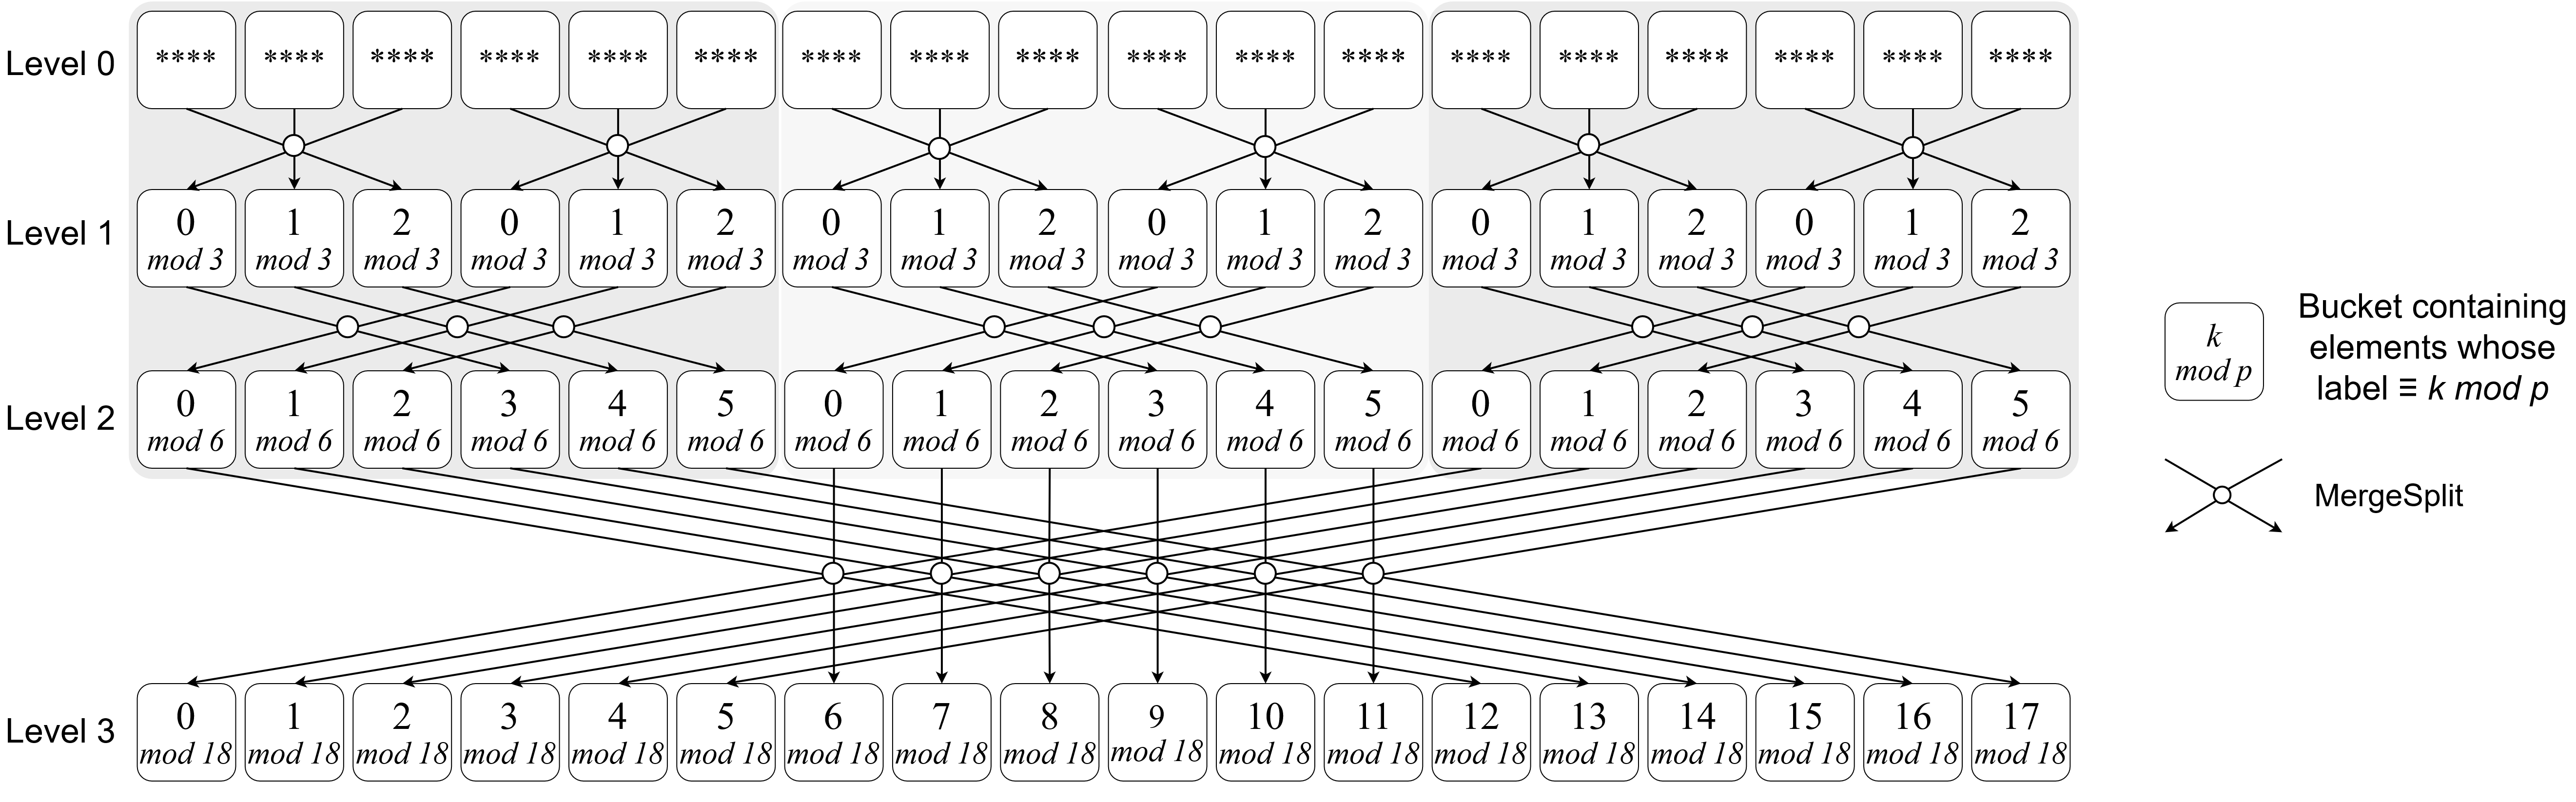
\includegraphics[width=\linewidth]{assets/multi-way-butterfly.png}
          \caption{A Multi-way Butterfly Network}
        \end{figure}
      \end{block}

    \end{column}

    % Second column
    \begin{column}{.30\linewidth}

      \begin{block}{Parallelism Abstraction}
        \begin{itemize}
          \item Across merge-split task in each batch
          \item Within each merge-split task
          \item Parallel External Merge Sort
          \item Parallel I/O
        \end{itemize}
      \end{block}

      \begin{block}{Parallelism in I/O}
        \begin{itemize}
          \item \textbf{Parallelism in I/O:} Identified three I/O patterns and used different strategies for parallelization.
          \item \textbf{Parallelism in Element Movement:} Utilized SIMD for parallelizing data movement, especially for elements with large payloads.
          \item \textbf{Parallelism in Pseudo-Random Numbers Generation:} Parallel generation of secure pseudo-random numbers using multiple generators.
        \end{itemize}
      \end{block}

    

      \begin{block}{Implementation}
        \begin{itemize}
          \item \textbf{Overview:} Implemented algorithm based on open-source code [5]. Modifications for parallelism and optimizations for high-end servers and consumer-grade processors.
          \item \textbf{Parallelize Butterfly Network:} Applied OpenMP directives for parallelization, changed routing schedule to iterative, and optimized parameters for maximum parallelism.
          \item \textbf{Parallelize I/O:} Identified three I/O patterns and used different strategies for parallelization.
          \item \textbf{Parallelize Element Movement:} Utilized SIMD for parallelizing element movement, applying C++ intrinsics with AVX512, AVX2, and SSE2 instruction sets.
          \item \textbf{Parallelize Pseudo-Random Number Generation:} Implemented multiple pseudo-random number generators for parallel generation.
          \item \textbf{Optimize Memory Utilization:} Addressed memory fragmentation concerns by allocating a memory pool and implementing a custom allocator.
        \end{itemize}
      \end{block}

    \end{column}
  

  % Third column
  \begin{column}{.30\linewidth}
    \begin{figure}
      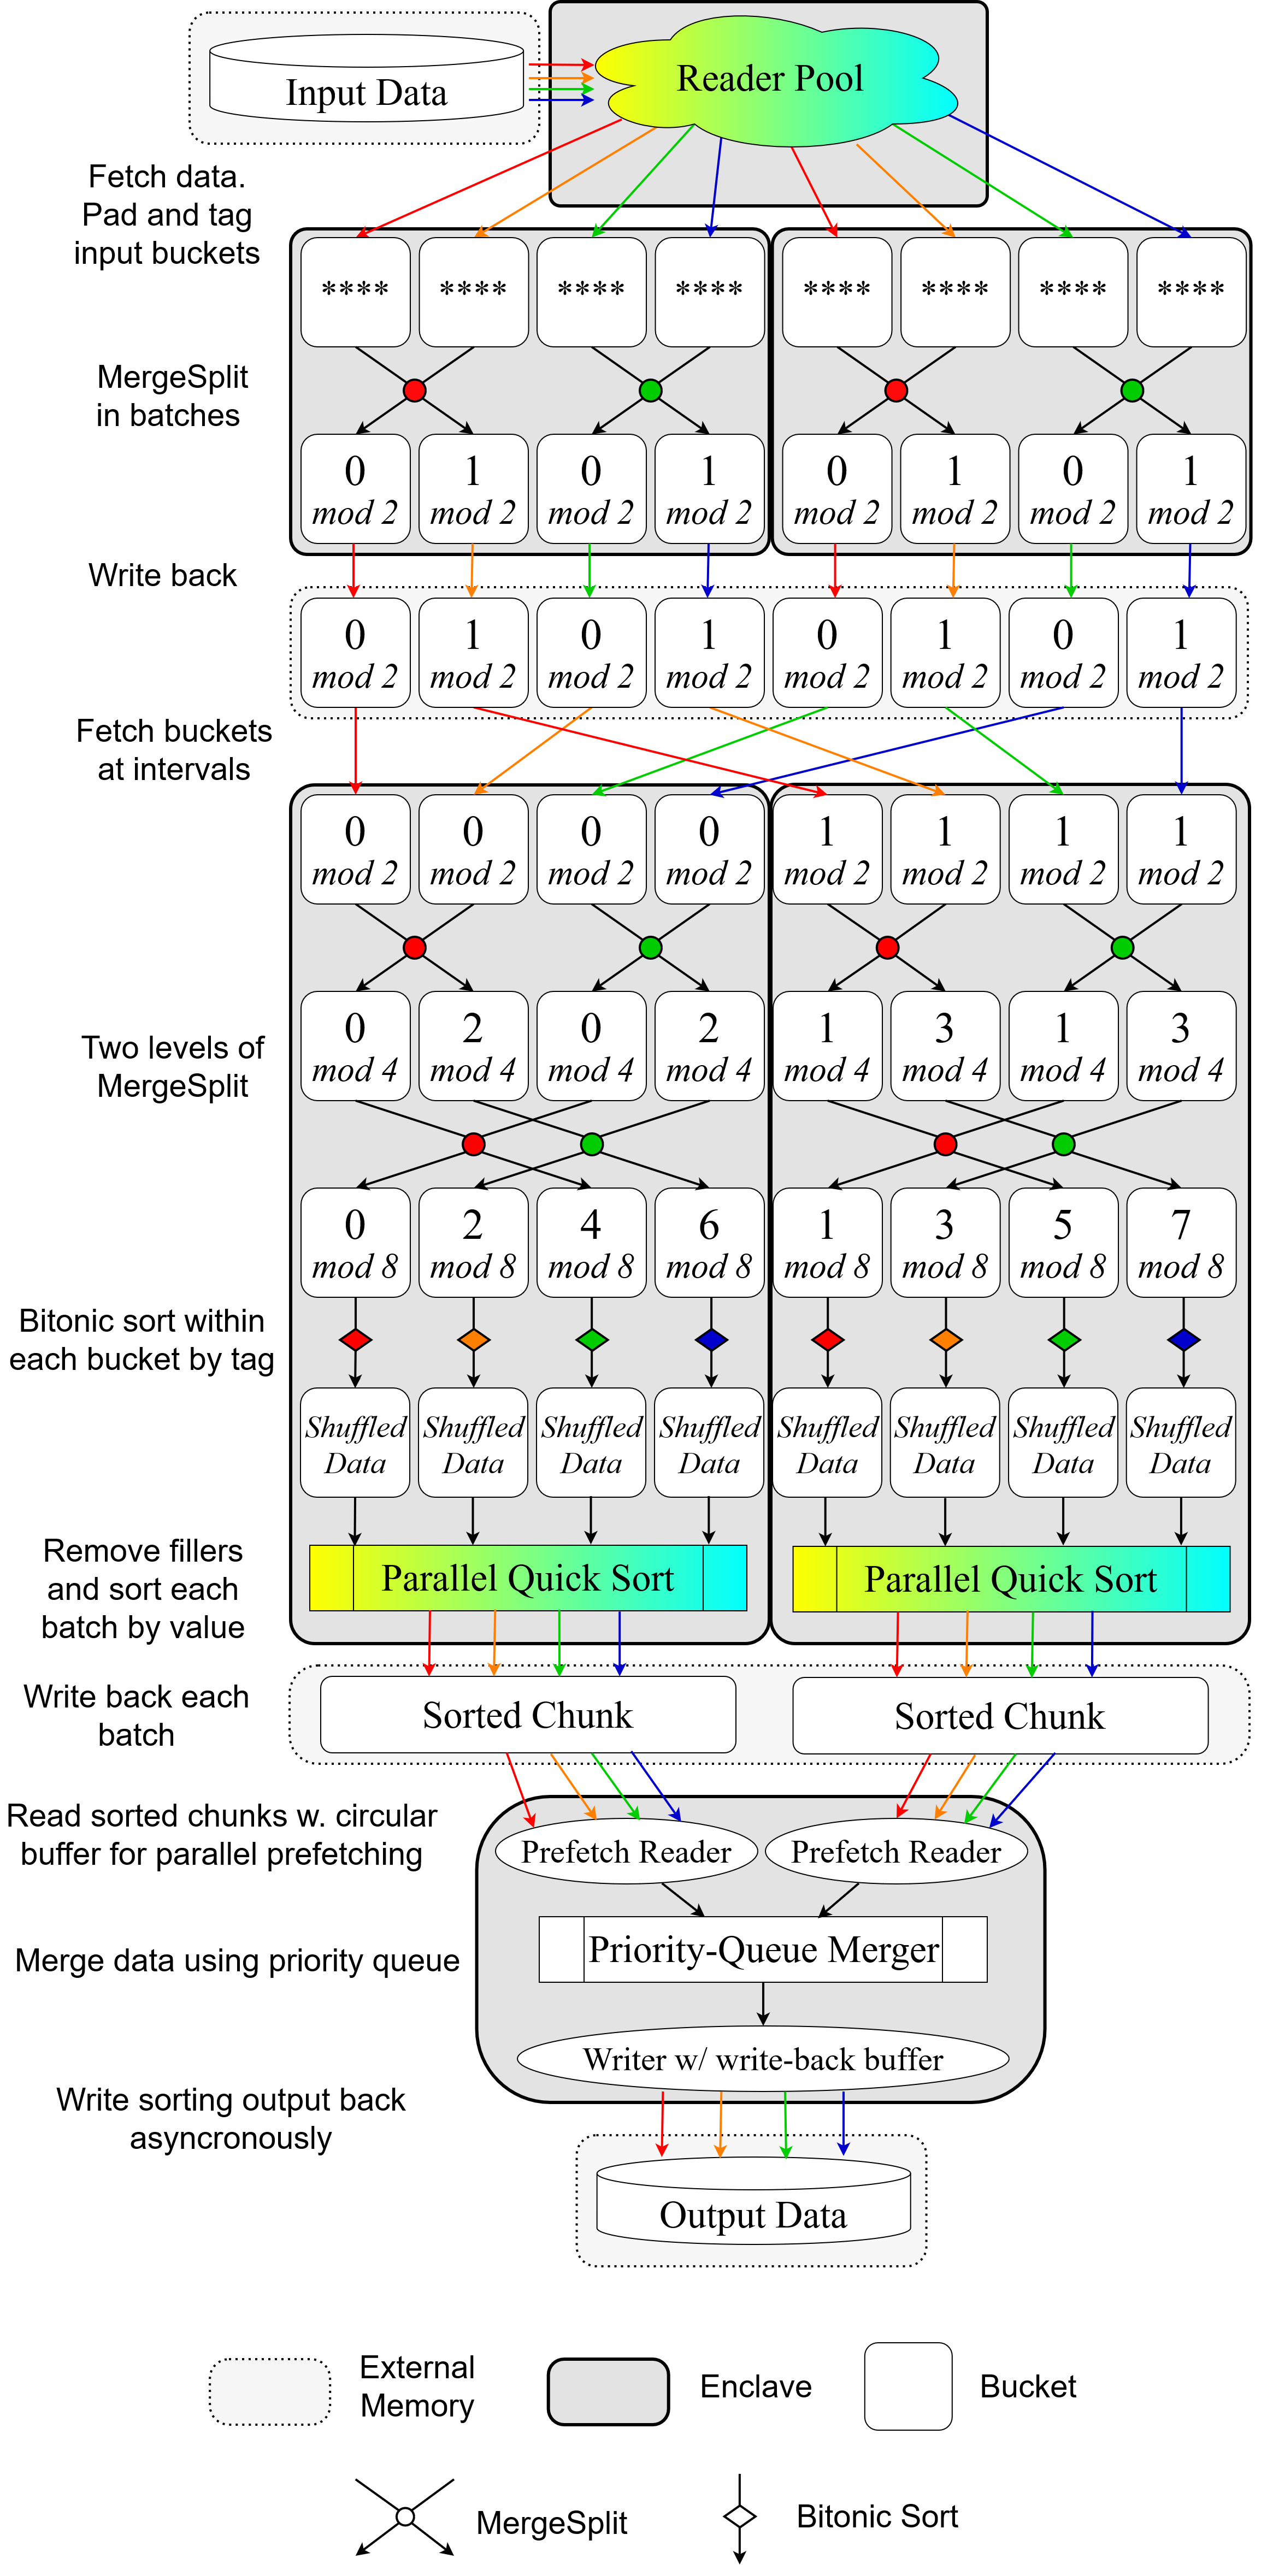
\includegraphics[width=\linewidth]{assets/parosort.png}
      \caption{Diagram of Parallel Oblivious Sort on a toy example. Each color represents a thread. Colorful components are multi-threaded.}
    \end{figure}
  \end{column}
  \end{columns}
\end{frame}
\end{document}